%%%%%%%%%%%%%%%%%%%%%%%%%%%%%%%%%%%%%%%%%
% Beamer Presentation
% LaTeX Template
% Version 1.0 (10/11/12)
%
% This template has been downloaded from:
% http://www.LaTeXTemplates.com
%
% License:
% CC BY-NC-SA 3.0 (http://creativecommons.org/licenses/by-nc-sa/3.0/)
%
%%%%%%%%%%%%%%%%%%%%%%%%%%%%%%%%%%%%%%%%%

%----------------------------------------------------------------------------------------
%	PACKAGES AND THEMES
%----------------------------------------------------------------------------------------

\documentclass{beamer}
\graphicspath{{Figures/}}
\usepackage[utf8]{inputenc}  % Para codificación de texto UTF8.
\usepackage[spanish]{babel}  % Para escritura en castellano.
\usepackage{xcolor}
\usepackage{subfigure}  % Para manejo de subfiguras.
\usefonttheme[onlymath]{serif}  

\mode<presentation> {

% The Beamer class comes with a number of default slide themes
% which change the colors and layouts of slides. Below this is a list
% of all the themes, uncomment each in turn to see what they look like.

%\usetheme{default}
%\usetheme{AnnArbor}
%\usetheme{Antibes}
%\usetheme{Bergen}
%\usetheme{Berkeley}
%\usetheme{Berlin}
%\usetheme{Boadilla}
%\usetheme{CambridgeUS}
%\usetheme{Copenhagen}
%\usetheme{Darmstadt}
%\usetheme{Dresden}
%\usetheme{Frankfurt}
%\usetheme{Goettingen}
%\usetheme{Hannover}
%\usetheme{Ilmenau}
%\usetheme{JuanLesPins}
%\usetheme{Luebeck}
\usetheme{Madrid}
%\usetheme{Malmoe}
%\usetheme{Marburg}
%\usetheme{Montpellier}
%\usetheme{PaloAlto}
%\usetheme{Pittsburgh}
%\usetheme{Rochester}
%\usetheme{Singapore}
%\usetheme{Szeged}
%\usetheme{Warsaw}

% As well as themes, the Beamer class has a number of color themes
% for any slide theme. Uncomment each of these in turn to see how it
% changes the colors of your current slide theme.

%\usecolortheme{albatross}
%\usecolortheme{beaver}
%\usecolortheme{beetle}
%\usecolortheme{crane}
%\usecolortheme{dolphin}
%\usecolortheme{dove}
%\usecolortheme{fly}
%\usecolortheme{lily}
%\usecolortheme{orchid}
%\usecolortheme{rose}
%\usecolortheme{seagull}
%\usecolortheme{seahorse}
%\usecolortheme{whale}
%\usecolortheme{wolverine}

%\setbeamertemplate{footline} % To remove the footer line in all slides uncomment this line
%\setbeamertemplate{footline}[page number] % To replace the footer line in all slides with a simple slide count uncomment this line

\setbeamertemplate{navigation symbols}{} % To remove the navigation symbols from the bottom of all slides uncomment this line
}

\usepackage{graphicx} % Allows including images
\usepackage{booktabs} % Allows the use of \toprule, \midrule and \bottomrule in tables
\renewcommand{\vec}[1]{\boldsymbol{#1}}
%----------------------------------------------------------------------------------------
%	TITLE PAGE
%----------------------------------------------------------------------------------------

\title[Tesis de grado]{Estudio de estructuras de banda prohibida electromagnética (EBG) para la reducción de acoplamiento mutuo entre antenas \textit{microstrip}} % The short title appears at the bottom of every slide, the full title is only on the title page

\author{Federico Luna} % Your name
\institute[] % Your institution as it will appear on the bottom of every slide, may be shorthand to save space
{
Facultad de Ingeniería,\\
Universidad de Buenos Aires \\ % Your institution for the title page
\medskip
\textit{fluna@fi.uba.ar}\\
\medskip % Your email address
Tutores: Dr. Ing. W. Gustavo Fano y Mg. Ing. Silvina Boggi
}
\date{} % Date, can be changed to a custom date

\begin{document}

\begin{frame}
\titlepage % Print the title page as the first slide
\end{frame}

\begin{frame}
\frametitle{Resumen} % Table of contents slide, comment this block out to remove it
\tableofcontents[hideallsubsections] % Throughout your presentation, if you choose to use \section{} and \subsection{} commands, these will automatically be printed on this slide as an overview of your presentation
\end{frame}

%----------------------------------------------------------------------------------------
%	PRESENTATION SLIDES
%----------------------------------------------------------------------------------------

%------------------------------------------------
\section{Presentación del problema} % Sections can be created in order to organize your presentation into discrete blocks, all sections and subsections are automatically printed in the table of contents as an overview of the talk
%------------------------------------------------
		\begin{frame}
			\frametitle{Objetivo}
			
			\begin{itemize}
				\item Propagación de ondas de superficie.
				\item Estructuras periódicas.
				\item Comportamiento de EBGs uniplanares.
				\item Modelo circuital equivalente de una celda unitaria.
				\item Programa de simulación en el dominio del tiempo.
				\item Introducción al uso de EBGs en antenas.
			\end{itemize}
		\end{frame}
	
		\begin{frame}
		\frametitle{Reseña histórica}
		\begin{itemize}
			\item 1873: \textit{Maxwell}. Bases de teoría electromagnética clásica.\\
			\item 1885-1887: \textit{Heaviside}. Simplificación de expresiones: Notación vectorial. \\
			\item 1886-1891: \textit{Hertz}. Validación de teoría de ondas electromagnéticas. Primer antena dipolo y parabólica.
			\item 1897: \textit{Rayleigh}. Propagación de ondas en guías metálicas.
			\item 1926: \textit{Yagi-Uda}. Conjunto de antenas, fase fija.
			\item 1938-1945: Antenas de fase variable.
			\item 1953: \textit{Deschamps}. Antenas \textit{microstrip}.
			\item 1970': Uso en aplicaciones prácticas. Solución a problemas de dispersión y modos indeseados.
			% Sustratos con bajas tangentes de pérdida. Mejora en fotolitografía. Optimización de modelos teóricos, simulaciones numéricas. Simplificación constructiva, más barato.
		\end{itemize}
		\end{frame}
	
		\begin{frame}
		\frametitle{Ventajas de las estructuras \textit{microstrip}}
		
		\begin{columns}[c] % The "c" option specifies centered vertical alignment while the "t" option is used for top vertical alignment
			
			\column{.50\textwidth} % Left column and width
			\begin{figure}[h]
				\centering
				\includegraphics[width=1\textwidth]{Presentacion/microstrip_general.pdf}
			\end{figure}
			
			\column{.45\textwidth} % Right column and width
			\begin{itemize}
				\item Bajo costo.
				\item Bajo peso.
				\item Construcción sencilla (fotolitografía).
				\item Cómodas para implantación de componentes discretos.
				\item Alto Q (resonantes).
			\end{itemize}
		
		\end{columns}
	
	\vspace{25pt}
	
	Aplicaciones: filtros microondas, acopladores direccionales, transformadores de impedancia, planos de tierra y redes de distribución de circuitos impresos.
		
	\end{frame}
		
		\begin{frame}
		\frametitle{Problemas de las estructuras \textit{microstrip}}
			El tamaño de las antenas y estructuras \textit{microstrip} depende de la permitividad dieléctrica del sustrato y de la longitud de onda de trabajo. \\
			\begin{columns}[c] % The "c" option specifies centered vertical alignment while the "t" option is used for top vertical alignment
				
				\column{.38\textwidth} % Left column and width
				
				\begin{itemize}
					\item $\downarrow D \Rightarrow \uparrow \epsilon_r,$ {\color{red}$\uparrow$ SW}.
					\item $\uparrow \epsilon_r \Rightarrow \uparrow Q, \downarrow$ BW.
					\item $\downarrow Q \Rightarrow \uparrow h$.
					\item $\uparrow h \Rightarrow ${\color{red}$\uparrow$ SW}, $\uparrow$ modos.
				\end{itemize}
				\vspace{5pt}
				Las ondas de superficie:
				\begin{itemize}
					\item $\downarrow$ potencia radiada.
					\item {\color{red}$\uparrow$ acoplamiento.}
					\item Diagrama de radiación: \\$\uparrow$ lóbulos secundarios. %Por discontinuidades
				\end{itemize}
				
				
				\column{.60\textwidth} % Right column and width
				\begin{figure}[h]
					\centering
					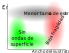
\includegraphics[width=1\textwidth]{Presentacion/problema_microstrip.pdf}
				\end{figure}
				
			\end{columns}
			\vspace{9pt}
			{\footnotesize SW: Ondas de superficie. BW: Ancho de banda. $D$: Tamaño de la estructura. $h$: Ancho del sustrato.}
		\end{frame}
		
		
		% Acá la idea es comentar que en general uno busca disminuir el tamaño. Eempezando de la esquina inferior derecha, uno tiene una estructura grande y fuerte. La quiere achicar, sale de la zona verde, hay mas ondas de superficie, y para bajar esas ondas no queda otra que bajar el ancho del sustrato, generando mayor fragilidad estructural. Modos indeseados.
		\begin{frame}
		\frametitle{Soluciones propuestas en la literatura}
		
		\begin{itemize}
			\item Separación del plano de tierra de las estructuras.
			\item Modificar la altura o la permitividad del sustrato a corta distancia.
			\item Estructuras periódicas: EBG, DGS.
		\end{itemize}
		
		\begin{figure}[H]
			\centering 
			\subfigure{
				\label{fig:sustrato-antena-ebg}
				\includegraphics[width=0.40\textwidth]{Aplicacion/foto-ebg-alrededor-antena.pdf}}
			\hspace{10pt}
			\subfigure{
				\label{fig:escalon-sustrato}
				\includegraphics[width=0.40\textwidth]{Aplicacion/foto-escalon-alrededor-antena.pdf}}
		\end{figure}
		\tiny{F. Yang e Y. Rahmat-Samii, Electromagnetic Band Gap Structures in Antenna Engineering, Cambridge University Press, 2009.}
		\end{frame}

\section{Conceptos básicos de electromagnetismo}

	\subsection{Ecuaciones de Maxwell} % A subsection can be created just before a set of slides with a common theme to further break down your presentation into chunks
	
		\begin{frame}
		\frametitle{Ecuaciones de Maxwell}
		
		\begin{align*}
		\left.\begin{array}{rr@{\mskip\thickmuskip}l}
		\text{Faraday} &\nabla \times \vec{E} & = -\frac{\partial \vec{B}}{\partial t} - \vec{M}\\
		\text{Ampère} &\nabla \times \vec{H} & = \frac{\partial \vec{D}}{\partial t} + \vec{J} \\
		\text{Gauss} &\nabla \cdot \vec{D} & = \rho \\
		\text{Gauss} & \nabla \cdot \vec{B} & = 0
		\end{array} \right\}
		\quad \implies \quad
		\left\{\begin{array}{r@{\mskip\thickmuskip}l}
		\nabla \times \vec{E} & = -j \omega \vec{B} - \vec{M} \\
		\nabla \times \vec{H} & = j \omega \vec{D} + \vec{J} \\
		\nabla \cdot \vec{D} & = \rho\\
		\nabla \cdot \vec{B} & = 0
		\end{array}\right.
		\end{align*}
		
		\begin{columns}[c] % The "c" option specifies centered vertical alignment while the "t" option is used for top vertical alignment
			
			\column{.62\textwidth} % Left column and width
			
			Si:
			\begin{itemize}
				\item No hay dispersión. ($\epsilon$ y $\mu$ independientes de $\omega$).
				\item Material isotrópico.
				\item Estudio macroscópico.
				\item Comportamiento armónico.
				\item Régimen permanente.
			\end{itemize}
			
			\column{.35\textwidth} % Right column and width
			\begin{figure}[h]
				\centering
				\includegraphics[width=1\textwidth]{Presentacion/James_Clerk_Maxwell.png}
			\end{figure}
			
		\end{columns}
				
		
		
		\end{frame}
		
		\begin{frame}
		\frametitle{Campos en medios materiales}
		Si el medio es lineal, isotrópico y homogéneo: %Si anisotrópico, Xe variaría con la dir. Si inhomogéneo, Xe variaría con la posición. Si no lineal, P debería calcularse como una serie de potencias.
		
		\begin{align*}
		\vec{D} = \epsilon_0 \vec{E} + \vec{P}_e = \epsilon_0 (1+\chi_e)\vec{E} = \epsilon \vec{E} &= (\epsilon' - j \epsilon'') \vec{E} y\\
		\vec{B} = \mu_0 (\vec{H} + \vec{P}_m) = \mu_0 (1+\chi_m)\vec{H} = \mu \vec{H} &= (\mu' - j \mu'') \vec{H}.
		\end{align*}
		
		Si el material posee una conductividad $\sigma$ independiente del campo eléctrico aplicado, se cumple la Ley de Ohm:
		
		\begin{align*}
		\vec{J} &= \sigma \vec{E} \Rightarrow \vec{D} = \left( \epsilon' - j\epsilon'' - j \frac{\sigma}{\omega} \right) \vec{E}.
		\end{align*}
		
		La tangente de pérdidas queda definida como:
		
		\begin{align*}
		\tan \; \delta &= \frac{\omega \epsilon'' + \sigma}{\omega \epsilon'}.
		\end{align*}
		
		
		\end{frame}
		
		\begin{frame}
		\frametitle{Ondas electromagnéticas (I)}
		
		\begin{figure}[h]
			\centering
			
\includegraphics[width=1\textwidth]{Presentacion/onda_em.pdf}
		\end{figure}
		
		En una región libre de fuentes, se pueden deducir las ecuaciones de Helmholtz para ondas monocromáticas, a partir de las ecuaciones de Maxwell.
				
		\begin{align*}
		\left.\begin{array}{rr@{\mskip\thickmuskip}l}
		\nabla^2  \vec{E} + \gamma^2 \vec{E} &= 0\\
		\nabla^2 \vec{H} + \gamma^2 \vec{H}& = 0
		\end{array} \right\}
		\quad \implies \quad
		\left\{\begin{array}{r@{\mskip\thickmuskip}l}
		\vec{E}(x,y,z) &= \vec{E}_0 e^{\pm j \vec{\gamma}\cdot \vec{r}}. \\
		\vec{H}(x,y,z) &= \vec{H}_0 e^{\pm j \vec{\gamma}\cdot \vec{r}}.
		\end{array}\right.
		\end{align*}
			
		\begin{align*}
		\gamma &= -j\alpha + \beta = j\omega \sqrt{\mu (\epsilon'-j\epsilon'') - j \sigma \epsilon/\omega}.\\
		\vec{\gamma} &= \vec{\gamma}_x + \vec{\gamma}_y +\vec{\gamma}_z
		\end{align*}

		\end{frame}
	
		\begin{frame}
		\frametitle{Ondas electromagnéticas (II)}
		
		
		
		
		\end{frame}
		
		% Comparar Masters Eq con Shrodinger. Modos.
		\subsubsection{Ondas guiadas}
		
			\begin{frame}
			\frametitle{Guías de onda}
			\end{frame}
	
			\begin{frame}
			\frametitle{Líneas de transmisión}
			\end{frame}
		
			\begin{frame}
			\frametitle{Líneas \textit{microstrip}}
			\end{frame}
		
		\subsubsection{Antenas}
		
			\begin{frame}
			\frametitle{Regiones de campo y diagrama de radiación}
			\end{frame}
		
			\begin{frame}
			\frametitle{Conjuntos de antenas y acoplamiento mutuo}
			\end{frame}
		
			\begin{frame}
			\frametitle{Antenas \textit{microstrip}}
			\end{frame}
		
			\begin{frame}
			\frametitle{Acoplamiento mutuo entre antenas \textit{microstrip}}
			\end{frame}
	
	
	\subsection{Ondas de superficie}
		\begin{frame}
		\frametitle{Reseña histórica y tipos de ondas de superficie}
		\end{frame}
		
		\subsubsection{Ondas de Zenneck}
			
			\begin{frame}
			\frametitle{Planteo matemático}
			\end{frame}
		
			\begin{frame}
			\frametitle{Constantes de propagación y atenuación: TM}
			\end{frame}	
		
			\begin{frame}
			\frametitle{Constantes de propagación y atenuación: TE}
			\end{frame}
		
		\subsubsection{Recubrimiento dieléctrico}
			
			\begin{frame}
			\frametitle{Planteo matemático}
			\end{frame}
			
			\begin{frame}
			\frametitle{Impedancia de superficie}
			\end{frame}
		

\begin{frame}
\frametitle{Paragraphs of Text}
El objetivo del trabajo es el estudio teórico y numérico del funcionamiento de estructuras EBG (\textit{Electromagnetic Bandgap}).\\~\\

Sed diam enim, sagittis nec condimentum sit amet, ullamcorper sit amet libero. Aliquam vel dui orci, a porta odio. Nullam id suscipit ipsum. Aenean lobortis commodo sem, ut commodo leo gravida vitae. Pellentesque vehicula ante iaculis arcu pretium rutrum eget sit amet purus. Integer ornare nulla quis neque ultrices lobortis. Vestibulum ultrices tincidunt libero, quis commodo erat ullamcorper id.
\end{frame}

%------------------------------------------------

\begin{frame}
\frametitle{Bullet Points}
\begin{itemize}
\item Lorem ipsum dolor sit amet, consectetur adipiscing elit
\item Aliquam blandit faucibus nisi, sit amet dapibus enim tempus eu
\item Nulla commodo, erat quis gravida posuere, elit lacus lobortis est, quis porttitor odio mauris at libero
\item Nam cursus est eget velit posuere pellentesque
\item Vestibulum faucibus velit a augue condimentum quis convallis nulla gravida
\end{itemize}
\end{frame}

%------------------------------------------------

\begin{frame}
\frametitle{Blocks of Highlighted Text}
\begin{block}{Block 1}
Lorem ipsum dolor sit amet, consectetur adipiscing elit. Integer lectus nisl, ultricies in feugiat rutrum, porttitor sit amet augue. Aliquam ut tortor mauris. Sed volutpat ante purus, quis accumsan dolor.
\end{block}

\begin{block}{Block 2}
Pellentesque sed tellus purus. Class aptent taciti sociosqu ad litora torquent per conubia nostra, per inceptos himenaeos. Vestibulum quis magna at risus dictum tempor eu vitae velit.
\end{block}

\begin{block}{Block 3}
Suspendisse tincidunt sagittis gravida. Curabitur condimentum, enim sed venenatis rutrum, ipsum neque consectetur orci, sed blandit justo nisi ac lacus.
\end{block}
\end{frame}

%------------------------------------------------

\begin{frame}
\frametitle{Multiple Columns}
\begin{columns}[c] % The "c" option specifies centered vertical alignment while the "t" option is used for top vertical alignment

\column{.45\textwidth} % Left column and width
\textbf{Heading}
\begin{enumerate}
\item Statement
\item Explanation
\item Example
\end{enumerate}

\column{.5\textwidth} % Right column and width
Lorem ipsum dolor sit amet, consectetur adipiscing elit. Integer lectus nisl, ultricies in feugiat rutrum, porttitor sit amet augue. Aliquam ut tortor mauris. Sed volutpat ante purus, quis accumsan dolor.

\end{columns}
\end{frame}

%------------------------------------------------



\section{Fundamentos de EBGs}

	\begin{frame}
	\frametitle{Reseña histórica}
	\end{frame}
	
	\subsection{Bragg, Bloch-Floquet y espacio recíproco}
	
		\begin{frame}
		\frametitle{Bragg}
		\end{frame}
	
		\begin{frame}
		\frametitle{Teorema de Bloch y armónicos espaciales}
		\end{frame}
	
		\begin{frame}
		\frametitle{Espacio recíproco}
		\end{frame}
	
	\subsection{Dispersión}
	
		\begin{frame}
		\frametitle{Dispersión en materiales comunes}
		\end{frame}
	
		\begin{frame}
		\frametitle{Representación de la dispersión en 2D}
		\end{frame}
	
		\begin{frame}
		\frametitle{Bandgap electromagnético}
		% Rods, TM, TE, combinación de los dos (Yablo), uso en waveguides. Dibujitos, senos deformes.
		\end{frame}
%------------------------------------------------

\begin{frame}
\frametitle{Table}
\begin{table}
\begin{tabular}{l l l}
\toprule
\textbf{Treatments} & \textbf{Response 1} & \textbf{Response 2}\\
\midrule
Treatment 1 & 0.0003262 & 0.562 \\
Treatment 2 & 0.0015681 & 0.910 \\
Treatment 3 & 0.0009271 & 0.296 \\
\bottomrule
\end{tabular}
\caption{Table caption}
\end{table}
\end{frame}

%------------------------------------------------

\begin{frame}
\frametitle{Theorem}
\begin{theorem}[Mass--energy equivalence]
$E = mc^2$
\end{theorem}
\end{frame}

%------------------------------------------------

\begin{frame}[fragile] % Need to use the fragile option when verbatim is used in the slide
\frametitle{Verbatim}
\begin{example}[Theorem Slide Code]
\begin{verbatim}
\begin{frame}
\frametitle{Theorem}
\begin{theorem}[Mass--energy equivalence]
$E = mc^2$
\end{theorem}
\end{frame}\end{verbatim}
\end{example}
\end{frame}

%------------------------------------------------

\begin{frame}
\frametitle{Figure}
Uncomment the code on this slide to include your own image from the same directory as the template .TeX file.
%\begin{figure}
%\includegraphics[width=0.8\linewidth]{test}
%\end{figure}
\end{frame}

%------------------------------------------------

\begin{frame}[fragile] % Need to use the fragile option when verbatim is used in the slide
\frametitle{Citation}
An example of the \verb|\cite| command to cite within the presentation:\\~

This statement requires citation \cite{p1}.
\end{frame}

%------------------------------------------------

\begin{frame}
\frametitle{References}
\footnotesize{
\begin{thebibliography}{99} % Beamer does not support BibTeX so references must be inserted manually as below
\bibitem[Smith, 2012]{p1} John Smith (2012)
\newblock Title of the publication
\newblock \emph{Journal Name} 12(3), 45 -- 678.
\end{thebibliography}
}
\end{frame}

%------------------------------------------------

\begin{frame}
\Huge{\centerline{The End}}
\end{frame}

%----------------------------------------------------------------------------------------

\section{Modelado}

	\subsection{Ecuación de dispersión}
		\begin{frame} % Need to use the fragile option when verbatim is used in the slide
		\frametitle{Ecuación de dispersión partir de una línea de transmisión}
		\end{frame}
	 
	 	\begin{frame} % Need to use the fragile option when verbatim is used in the slide
	 	\frametitle{Diagrama de dispersión}
 	    \end{frame}
      
     \subsection{Métodos numéricos}
	    \begin{frame} % Need to use the fragile option when verbatim is used in the slide
	    \frametitle{Métodos numéricos}
	 	\end{frame}
	
		\begin{frame} % Need to use the fragile option when verbatim is used in the slide
		\frametitle{Resultados de simulaciones para celda sencilla}
		\end{frame}
		
		\begin{frame} % Need to use the fragile option when verbatim is used in the slide
		\frametitle{Análisis de diagrama de dispersión típico}
		\end{frame}
		
	 \subsection{Análisis paramétrico de una celda sencilla}
	 
	 	\begin{frame} % Need to use the fragile option when verbatim is used in the slide
	 	\frametitle{Variación del ancho del puente}
 		\end{frame}
 	
	 	\begin{frame} % Need to use the fragile option when verbatim is used in the slide
	 	\frametitle{Variación del tamaño de la celda unitaria}
	 	\end{frame}
 	
	 	\begin{frame} % Need to use the fragile option when verbatim is used in the slide
	 	\frametitle{Variación del lado del parche}
	 	\end{frame}
 	
	 	\begin{frame} % Need to use the fragile option when verbatim is used in the slide
	 	\frametitle{Variación del ancho del sustrato}
	 	\end{frame}
 	
\section{Análisis y modelado de la celda de Yang}
		
		\begin{frame} % Need to use the fragile option when verbatim is used in the slide
		\frametitle{Celda de Yang}
		\end{frame}
	
		\begin{frame} % Need to use the fragile option when verbatim is used in the slide
		\frametitle{Comportamiento}
		\end{frame}
	
	\subsection{Construcción del modelo circuital}
		\begin{frame} % Need to use the fragile option when verbatim is used in the slide
		\frametitle{Modelo I}
		\end{frame}
	
		\begin{frame} % Need to use the fragile option when verbatim is used in the slide
		\frametitle{Modelo I: Resultados}
		\end{frame}
	
		\begin{frame} % Need to use the fragile option when verbatim is used in the slide
		\frametitle{Modelo II}
		\end{frame}

		\begin{frame} % Need to use the fragile option when verbatim is used in the slide
		\frametitle{Modelo II: Resultados}
		\end{frame}
		
		\begin{frame} % Need to use the fragile option when verbatim is used in the slide
		\frametitle{Modelo II: Diagrama de dispersión}
		\end{frame}
	
		\begin{frame} % Need to use the fragile option when verbatim is used in the slide
		\frametitle{Modelo III}
		\end{frame}
	
		\begin{frame} % Need to use the fragile option when verbatim is used in the slide
		\frametitle{Modelo III: Resultados}
		\end{frame}
	
		\begin{frame} % Need to use the fragile option when verbatim is used in the slide
		\frametitle{Modelo III: Diagrama de dispersión}
		\end{frame}
	
	\subsection{Comportamiento II}
		\begin{frame} % Need to use the fragile option when verbatim is used in the slide
		\frametitle{Comportamiento de una fila}
		\end{frame}
	
		\begin{frame} % Need to use the fragile option when verbatim is used in the slide
		\frametitle{Comportamiento de una estructura}
		\end{frame}
	
\section{Construcción del algoritmo de simulación en el dominio del tiempo}
		\begin{frame} % Need to use the fragile option when verbatim is used in the slide
		\frametitle{Definiciones}
		\end{frame}
	
		\begin{frame} % Need to use the fragile option when verbatim is used in the slide
		\frametitle{Resultados}
		\end{frame}

\end{document}